\section{Aufbau und Durchführung} % (fold)
\label{sec:durchfhrung}


In diesem Versuch wird die in %\ref{fig:drillachse} 
gezeigte Apparatur verwendet: 
Eine drehbar gelagerte Achse ist über eine Spiralfeder an einen festen Rahmen gekoppelt. 
In das obere Ende der Drillachse können verschiedene Körper eingespannt werden; 
in %\ref{fig:drillachse} 
vertreten durch die Kugel. 
[ Unterhalb des Körpers befindet sich ein Auslenkungswinkelskalaablesdingsbums. ]


%\begin{figure}
	% \label{fig:drillachse}
	% \caption{Skizze des Versuchsaufbaus. Eine drehbar gelagerte Drillachse mit Spiralfeder im festen Rahmen mit Befestigung für die Probekörper hier eine Kugel.}
	% \centering
	% 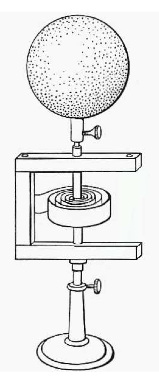
\includegraphics[height=7cm]{drillachse}
% \end{figure}

\subsection{Bestimmung der Winkelrichtgröße $D$}
Zur Bestimmung der Winkelrichtgröße $D$ wird eine im folgenden als masselos angenommene Metallstange mittig und senkrecht zur Drehachse in die Vorrichtung eingespannt, 
sodass die Drehachse durch den Stangenschwerpunkt verläuft. 
Eine im Abstand $r$ zum Drehzentrum angehängte Federwaage misst die Kraft $F$ des rücktreibenden Drehmomentes bei Auslenkung der Metallstange um einen bestimmten Winkel $\phi$. 
Zu beachten ist, dass die Federwaage bestenfalls senkrecht zum Stab und zur Rotationsachse gehalten wird. 
Dadurch kann der Betrag des Drehmoments $M$ durch
\begin{equation}
	| \vec{M} | = | \vec{r} \times \vec{F} | = r F \sin (\angle({\vec{r}}),
	\vec{F}) = r F
\end{equation}
berechnet werden.
Diese Messung wird für 10 verschiedene Winkel $\phi$ zwischen 0 und $2\mathup{\pi}$ durchgeführt. 
%[Unnötig?..Neben der zuvor beschriebenen statischen Methode kann D auch über die gemessene Schwingungsdauer T mit Formel (NUMMER) berechnet werden. Diese dynamische Methode wird jedoch nicht angewandt.]

\subsection{Bestimmung des Eigenträgheitsmomentes $I_{\mathup{D}}$ der Drillachse}
Auf die Metallstange aus Kapitel 2.1 wird links und rechts des Drehzentrums je eine als punktförmig angesehene Masse befestigt, deren Abstand $a$ zum Stangenschwerpunkt variabel ist. 
Nun wird die Stange ausgelenkt und mit einer Stoppuhr die Schwingungsdauer $T$ für 5 Perioden gemessen. 
Das Verfahren wird für 9 weitere Messwerte wiederholt, wobei vor jeder Messung einer neuer Abstand $a$ eingestellt und notiert wird. 
Zu beachten ist, dass die links- und rechtsseitige Masse gleichweit vom Mittelpunkt entfernt sind. 
Im Anschluss an die Messung der Schwingungsdauer werden Gewicht und Abmessungen der Massen mit Waage und Schieblehre bestimmt.

\subsection{Bestimmung der Trägheitsmomente verschiedener Körper}
Als erster Körper wird ein Styroporzylinder gewählt, welcher senkrecht auf die Drillachse gesteckt wird, 
nachdem sowohl die Massen, als auch die Metallstange aus vorherigen Messungen von der Apparatur geschraubt wurden. 
Anschließend wird dieser ebenfalls zur Schwingung gebracht und die Schwingungsdauer $T$ für 5 Schwingungen insgesamt 10 Mal gemessen. 
Das Verfahren wiederholt sich für die Kugel, den zweiten Körper. 
Auch diese Körper werden nach der Messung gewogen und mit einer Schieblehre vermessen - Länge und Durchmesser des Zylinders, als auch Durchmesser der Kugel. 

\subsection{Bestimmung der Trägheitsmomente der Modellpuppe für 2 verschiedene Positionen}
Die Puppe wird in die Messvorrichtung eingespannt und in Position (a), abgebildet in %\ref{fig:Puppe},
gebracht. 
Der Messvorgang verläuft analog zu den vorherigen. 
Die Zeit $T$ für 5 Schwingungen wird 10 Mal mit einer Stoppuhr gemessen. 
Danach wird die Puppe in Position (b), ebenfalls in %\ref{fig:Puppe} 
ersichtlich, gebracht und erneut gemessen. 
Es folgen die Bestimmung des Gewichtes mit einer Waage und die Vermessung der einzelnen Körperteile der Puppe. 
Es werden Durchmesser und ggf. die Länge von Armen, Beinen, Kopf und Rumpf mit einer Schieblehre vermessen.

% section durchfhrung (end)
